Initial text before, like in human



\subsection{Bovine \textit{IFIT} Responses to Activators of Innate Immune Response} \label{subsec:Bovine IFIT Responses to Activators of Innate Immune Response}
some text here about what wrote prevoiusly


The Madin-Darby bovine kidney (MDBK) cell line, derived from bovine renal epithelium in 1958 (\cite{Madin1958EstablishedOrigin}), is an established model system used in bovine virology studies. We assayed them for the induction potential of bovine \textit{IFITs}, alongside bovine \textit{Mx1} using bovine interferon alpha and LPS (bovine interferon-gamma was not available commercially). Bovine \textit{Mx1} was included in the analyses as it is a ISG, widely reported in immunology and virology studies (ADD SOME REFERENCES HERE FOR CRYING OUT LOUD), and because we saw minimal bovine \textit{IFIT} responses throughout the study and wanted to ensure the cell lines used had the internal pathways for ISG induction correctly functioning. Figure \ref{fig:MDBK responses to bIFNa} shows the \textit{bIFIT} and \textit{bMx1} responses to the stimulation with bIFN\(\alpha\) at a concentration of 5 ng/mL (equivalent to 1,000 UI/mL of hIFN\(\alpha\)) for either 3 or 6 hours. Interestingly, we see a similar effect in induction amplitude but an opposing effect in time of stimulation to amplitude compared to hIFN\(\alpha\) induction in BEAS-2B cells (Figure \ref{fig:BEAS-2B responses to hIFNa}). DESCRIBE THE DATA ITSELF

Old text:
Alongside confirming the induction potential of bIFITs in MDBK cells, we assessed the effect of bovine respiratory syncytial virus (bRSV) on IFIT induction. As bRSV is a known inducer of the interferon response we expect bovine IFIT genes to be upregulated following infection. MDBK cells were infected with purified bRSV at MOI of 1 for 24 and 48 hours. As a positive control human IFNa was used. This was due to the unavailability of a bovine counterpart at that point, however, Gresser and his colleagues (1974), reported that hIFNa does indeed affect bovine cells as well. Cellular RNA was extracted and converted to complementary DNA, as described in section 7.3. Bovine IFIT transcripts were quantified relative to mock-infected cells. qPCR results (Figure 7A) were normalised to bovine GAPDH levels. We observed large variation in the transcriptional response, even in mock-infected cells. bIFITs 2, 3 and 5 mRNA levels did not change in response at any time point post bRSV infection. bIFIT1 was induced at 48 hours post-infection, but the variation is too high to make firm conclusions at this point. However, consistent with Gresser et al`s previous findings, bIFITs were responsive to 1000 units of hIFNa; all genes were highly induced (Figure 7B), although the fold expression increases varied greatly. bIFIT1 increased 10000-fold, followed by bIFIT2 and bIFIT3 with both having c. 700-fold increase. bIFIT5 mRNA expression was induced by c. 25-fold after treatment with hIFNa. This experiment was performed once and will be repeated. As a control for infection, quantification of viral RNA using qPCR will provide us with a clearer picture about the observed changes.


\begin{figure}
    \centering
    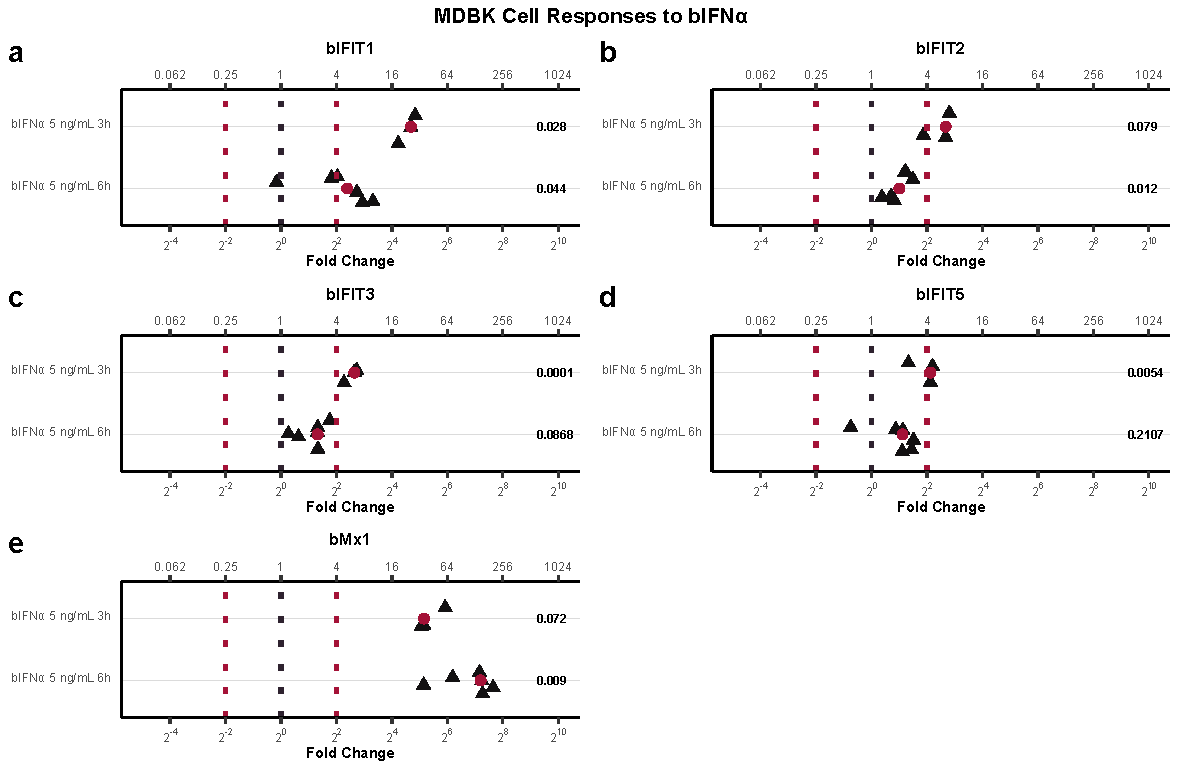
\includegraphics[width=1\linewidth]{07. Chapter 2/Figs/02. Induction/01. mdbk_treat_bifna.pdf}
    \caption[\textit{bIFIT} Gene Expression in MDBK Cells in Response to bIFN\(\alpha\) Stimulation.]{\textbf{\textit{bIFIT} Gene Expression in MDBK Cells in Response to bIFN\(\alpha\) Stimulation.} (a) \textit{bIFIT1}, (b) \textit{bIFIT2}, (c) \textit{bIFIT3}, (d) \textit{bIFIT5}, and (e) \textit{bMx1} gene expression levels were assessed using quantitative real-time PCR (qPCR) in MDBK cells following stimulation with bovine interferon alpha (IFN\(\alpha\)) at a concentration of 5 ng/mL for a treatment duration of either 3 or 6 hours. Relative expression values are normalized to standardized mock-treated samples. Median values are represented by red circles. The black dotted line represents mock expression levels, while the red dotted lines indicate biologically significant induction thresholds. Numeric values indicate the p-values compared to mock-treated samples.}
    \label{fig:MDBK responses to bIFNa}
\end{figure}


some text about bifn stimulation

\begin{figure}
    \centering
    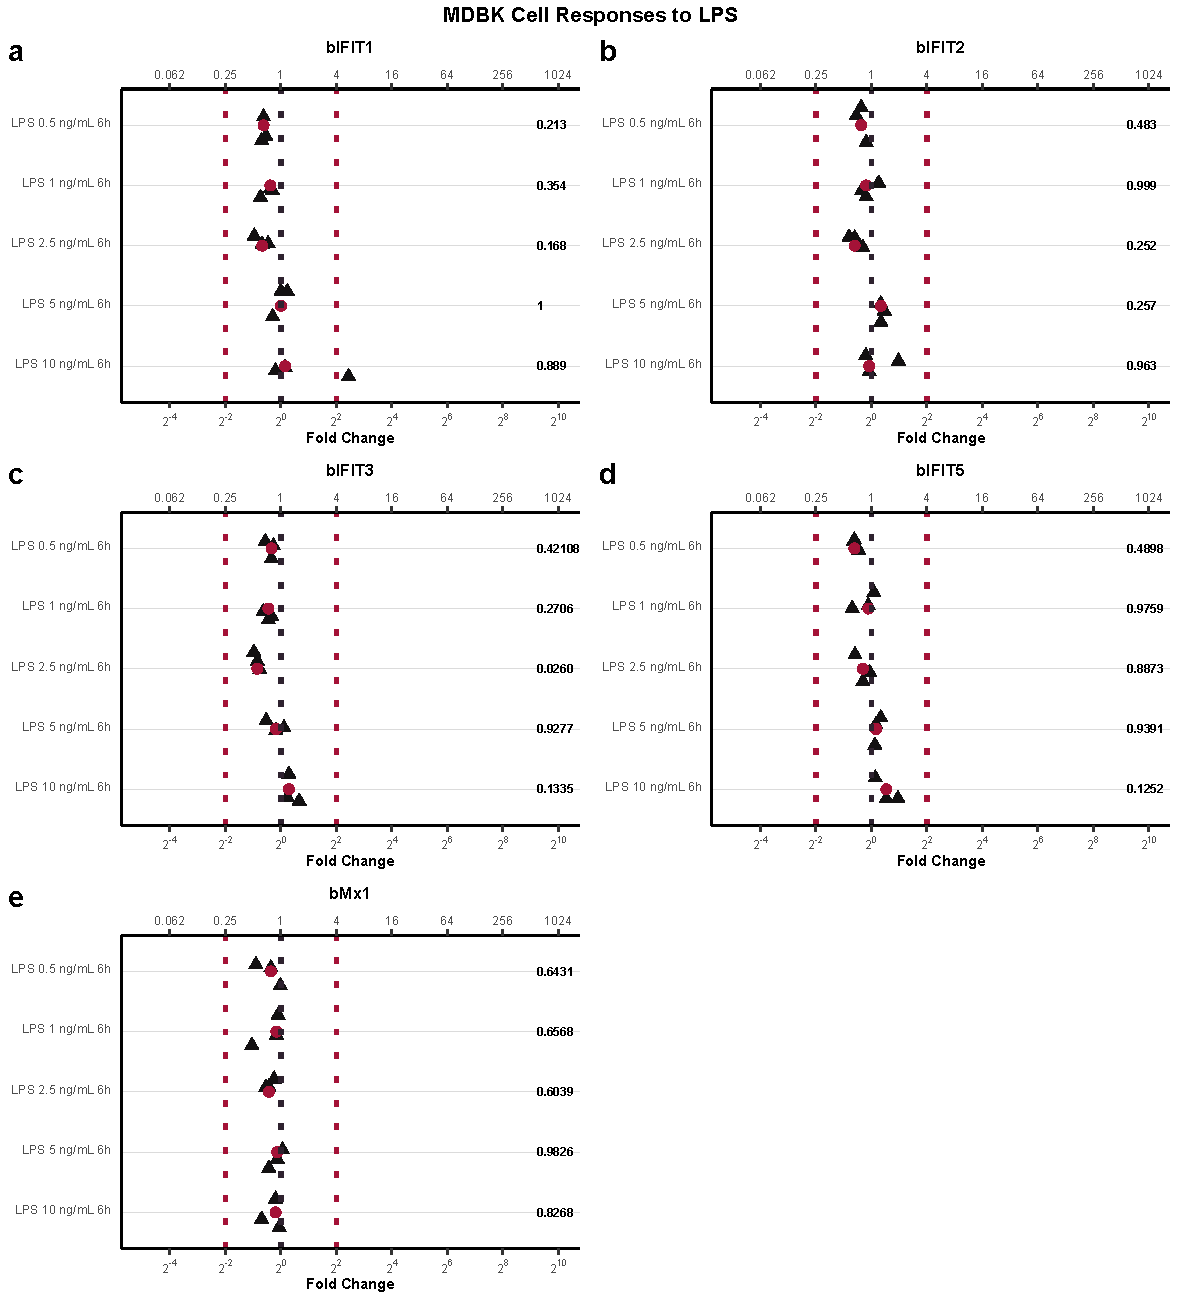
\includegraphics[width=1\linewidth]{07. Chapter 2/Figs/02. Induction/02. mdbk_treat_lps.pdf}
    \caption[\textit{bIFIT} Gene Expression in MDBK Cells in Response to LPS Stimulation.]{\textbf{\textit{bIFIT} Gene Expression in MDBK Cells in Response to LPS Stimulation.} (a) \textit{bIFIT1}, (b) \textit{bIFIT2}, (c) \textit{bIFIT3}, (d) \textit{bIFIT5}, and (e) \textit{bMx1} gene expression levels were assessed using quantitative real-time PCR (qPCR) in MDBK cells following stimulation with bacterial LPS at a concentration of 0.5, 1, 2.5, 5, and 10 ng/mL for a treatment duration of 6 hours. Relative expression values are normalized to standardized mock-treated samples. Median values are represented by red circles. The black dotted line represents mock expression levels, while the red dotted lines indicate biologically significant induction thresholds. Numeric values indicate the p-values compared to mock-treated samples.}
    \label{fig:MDBK responses to LPS}
\end{figure}


Bovine Mx1 is included in all experiments with bovine cells as it is an ISG that is induced by range of infections and the activators of innate immune response. It is also a control for bIFN alpha (if it works properly and is not degraded).

Neither bMx1 nor bIFITs are induced by LPS in the concentration range tested. bMx1 was induced by all bIFN alpha at different concentrations and timepoints, but at 5 ng/mL for 24h. This means that either that treatment failed or 24h post adding the bIFN treatment is too late to capture the ISG induction. All targets are induced by bIFN alpha treatment at 5 ng/mL for 3 hours. bIFIT1 also responds to low concentration (0.5 ng/mL) for 6h treatment, but not the other IFITs. No other concentration/time combination induced bIFITs. 

This all suggests that MDBK are responsive to bIFN alpha and capable of bIFIT induction, but the responses are week, especially compared to human cells.

I have a hypothesis that in bovine cells the IFITs are basally expressed to higher levels  (that would explain why we can detect them by IF in mock and infected cell although the qPCR data suggest there is no induction).


\begin{figure}
    \centering
    \caption[\textit{bIFIT} Gene Expression in BT Cells in Response to bIFN\(\alpha\) Stimulation.]{\textbf{\textit{bIFIT} Gene Expression in BT Cells in Response to bIFN\(\alpha\) Stimulation.} (a) \textit{bIFIT1}, (b) \textit{bIFIT2}, (c) \textit{bIFIT3}, (d) \textit{bIFIT5}, and (e) \textit{bMx1} gene expression levels were assessed using quantitative real-time PCR (qPCR) in BT cells following stimulation with bovine interferon alpha (IFN\(\alpha\)) at a concentration of 5 ng/mL for a treatment duration of either 3 or 24 hours. Relative expression values are normalized to standardized mock-treated samples. Median values are represented by red circles. The black dotted line represents mock expression levels, while the red dotted lines indicate biologically significant induction thresholds. Numeric values indicate the p-values compared to mock-treated samples.}
    \label{fig:BT responses to bifna}
\end{figure}


% bt paper
(\cite{McClurkin1974ComparisonVirus})


\subsection{Bovine \textit{IFITs} Responses to bRSV} \label{subsec:Bovine IFITs Responses to bRSV}

sdfasdfasdf


UV inactivated bRSV causes no change for bMx1 and bIFIT2 and seems to downregulate bIFIT1,3,5. Low, mid, and high MOI (0.1, 1, 2) and two different time points (24 and 48 HPI) do not seem to influence the levels of any genes tested other than for bMx1 for wt ultracentrifugation purified bRSV 24 HPI MOI 1. I have one experiment where bRSV MOI 1 24 HPI downregulates all genes tested but it might be a technical error. 
Very low MOI (0.001) wt bRSV along with MOI 1 dSH and very low MOI dNS1, dSN2 and dNS1/2 bRSV do not up or downregulate any genes tested in a biologically significant way.

\begin{figure}
    \centering
    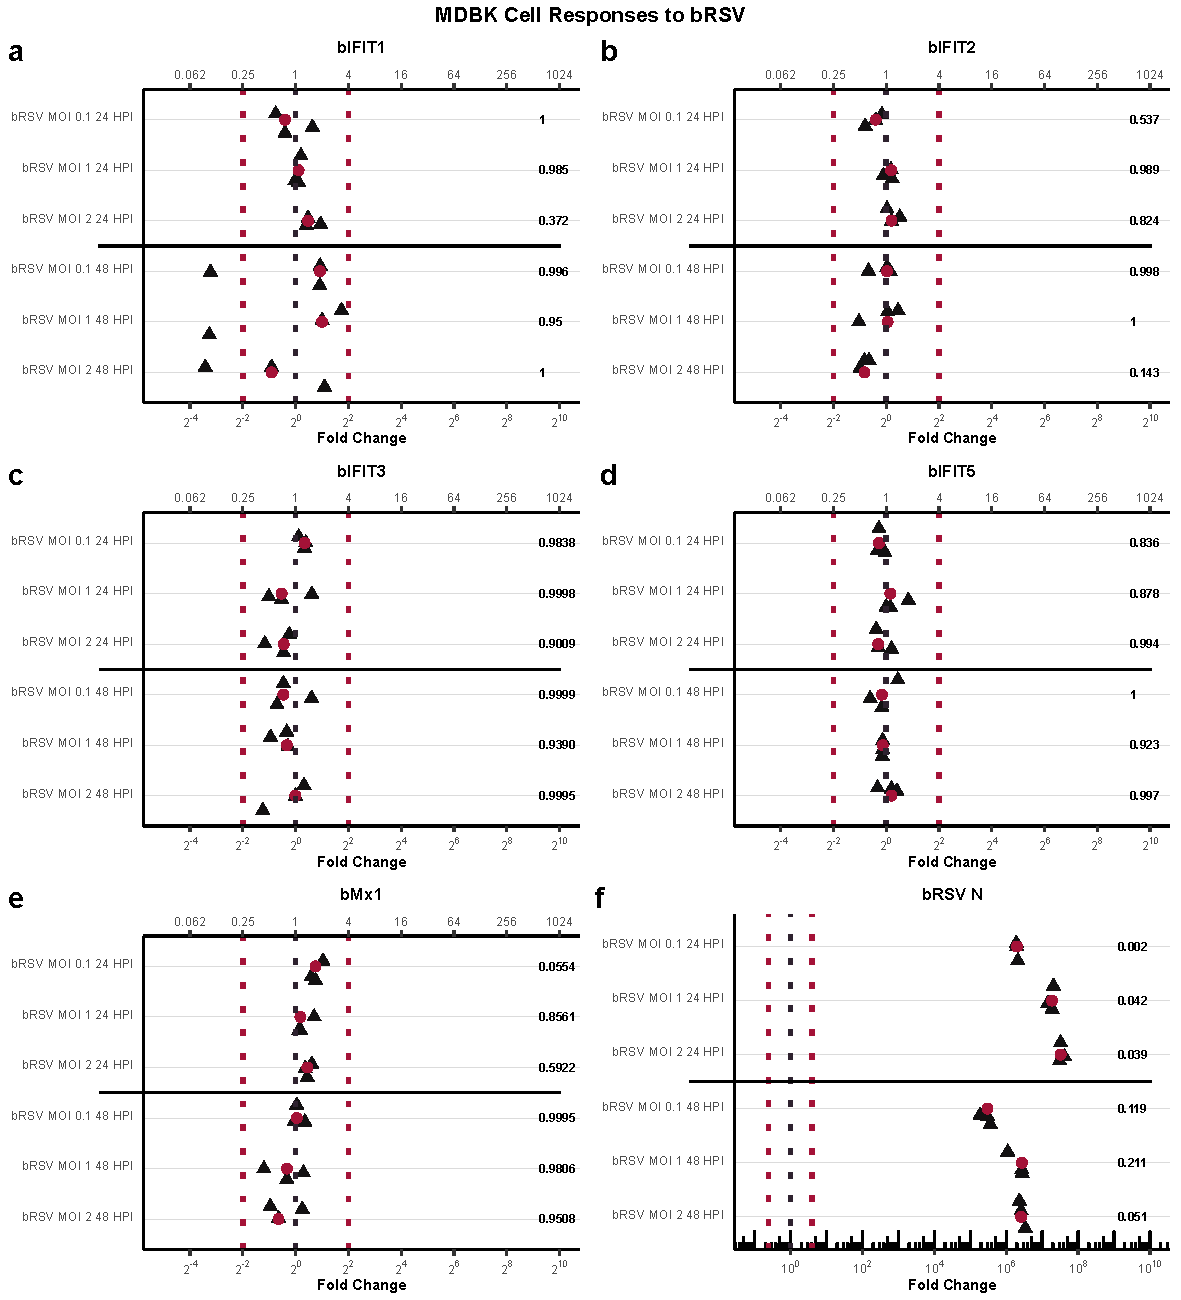
\includegraphics[width=1\linewidth]{07. Chapter 2/Figs/02. Induction/03. mdbk_brsv_timepoints.pdf}
    \caption[MDBK \textit{bIFIT} Response to bRSV Infection as a Function of Time and MOI.]{\textbf{MDBK \textit{bIFIT} Response to bRSV Infection as a Function of Time and MOI.} (a) \textit{bIFIT1}, (b) \textit{bIFIT2}, (c) \textit{bIFIT3}, (d) \textit{bIFIT5}, (e) \textit{bMx1} and (f) \textit{bRSV N} gene expression levels were assessed using quantitative real-time PCR (qPCR) in MDBK cell line following infection with bovine RSV at MOI of either 0.1, 1, or 2 for either 24 or 48 hours post-infection. Relative expression values are normalized to standardized mock-treated samples. Median values are represented by red circles. The black dotted line represents mock expression levels, while the red dotted lines indicate biologically significant induction thresholds. Numeric values indicate the p-values compared to mock-treated samples.}
    \label{fig:MDBK responses to bRSV timepoints}
\end{figure}

some text some text some text some text some text

\begin{figure}
    \centering
    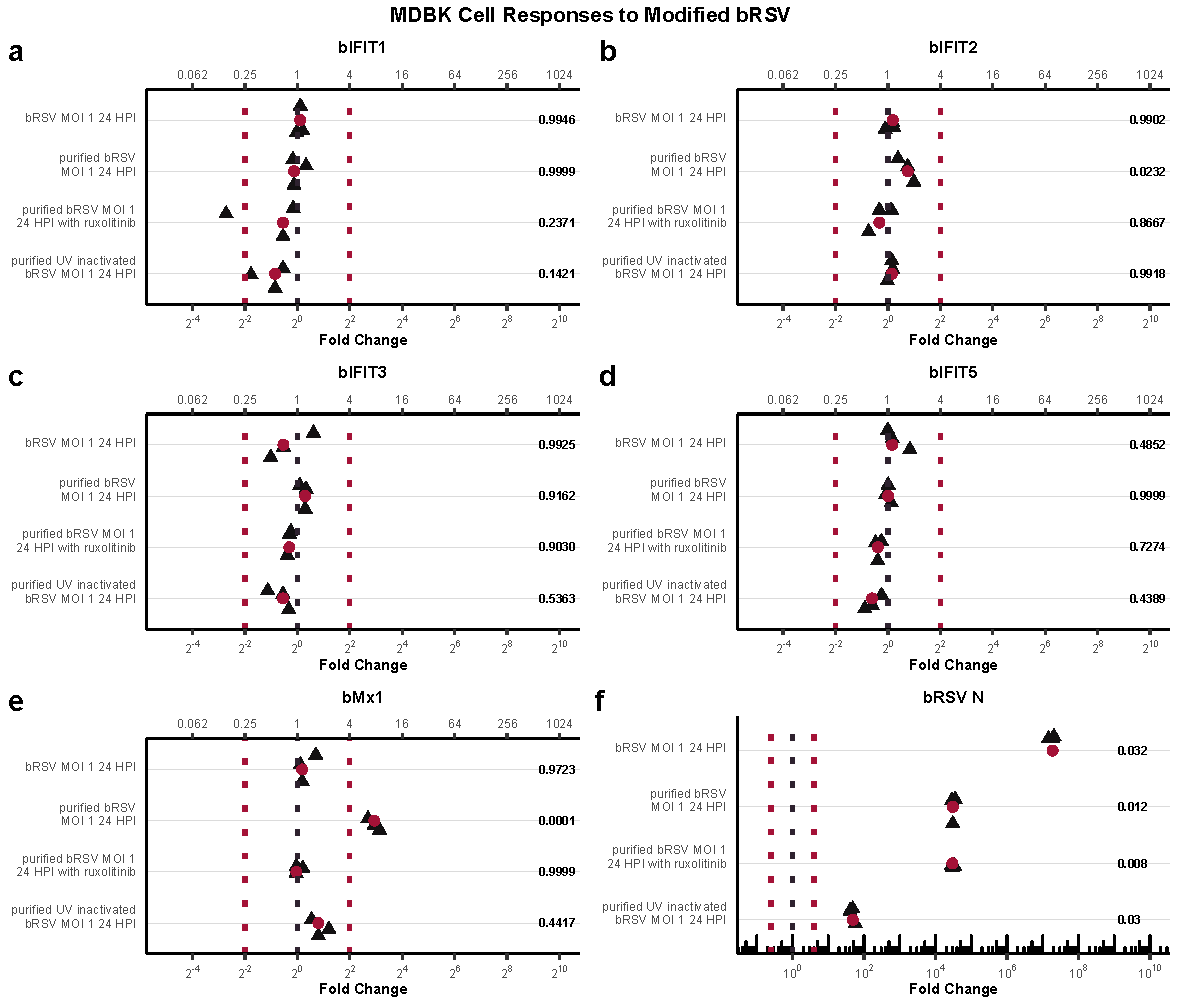
\includegraphics[width=1\linewidth]{07. Chapter 2/Figs/02. Induction/04. mdbk_brsv_uv_roxo.pdf}
    \caption[Impact of Ultra-Purification, UV-Inactivation, and INFR Inhibition on \textit{bIFIT} Induction in MDBK Cells Following bRSV Infection.]{\textbf{Impact of Ultra-Purification, UV-Inactivation, and INFR Inhibition on \textit{bIFIT} Induction in MDBK Cells Following bRSV Infection.} (a) \textit{bIFIT1}, (b) \textit{bIFIT2}, (c) \textit{bIFIT3}, (d) \textit{bIFIT5}, (e) \textit{bMx1}, and (f) \textit{bRSV N} gene expression levels were assessed using quantitative real-time PCR (qPCR) in MDBK cell line following infection with ultra-purified bRSV at MOI 1 for 24 hours. The cells were subjected to three different conditions: virus infection alone (top row), virus infection in the presence of 5 nM of ruxolitinib (interferon receptor inhibitor) throughout the infection (middle row), or UV-inactivated bRSV infection (bottom row). Relative expression values are normalized to standardized mock-treated samples. Median values are represented by red circles. The black dotted line represents mock expression levels, while the red dotted lines indicate biologically significant induction thresholds. Numeric values indicate the p-values compared to mock-treated samples.}
    \label{fig:The effect of ultra-purification, UV-inactivation and INFR inhibition on hIFIT induction following hRSV infection in MDBK}
\end{figure}


some text some text some text some text some text

\begin{figure}
    \centering
    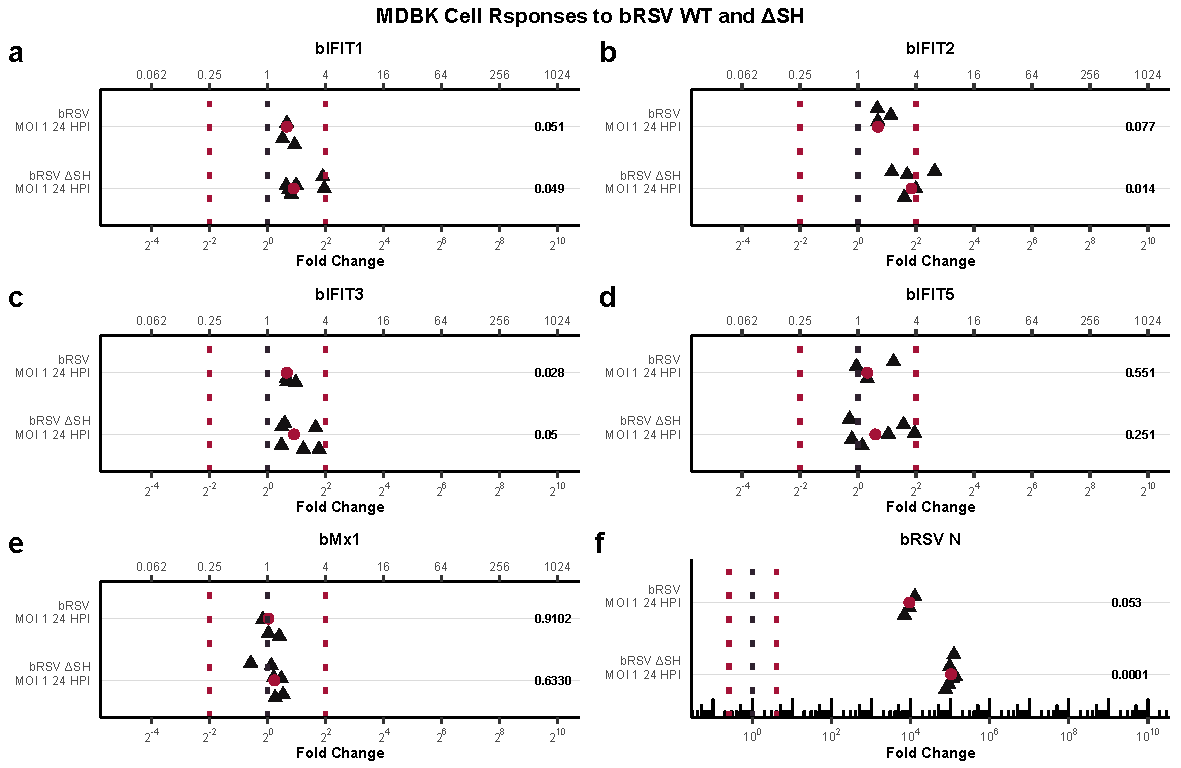
\includegraphics[width=1\linewidth]{07. Chapter 2/Figs/02. Induction/05. mdbk_brsv_moi1_dsh.pdf}
    \caption[MDBK \textit{bIFIT} Response to WT and \(\Delta\)SH bRSV Infection.]{\textbf{MDBK \textit{bIFIT} Response to WT and \(\Delta\)SH bRSV Infection.} (a) \textit{bIFIT1}, (b) \textit{bIFIT2}, (c) \textit{bIFIT3}, (d) \textit{bIFIT5}, (e) \textit{bMx1}, and (f) \textit{bRSV N} gene expression levels were assessed using quantitative real-time PCR (qPCR) in MDBK cell line following infection with WT or \(\Delta\)SH bRSV at MOI 1 for 24 hours post-infection. Relative expression values are normalized to standardized mock-treated samples. Median values are represented by red circles. The black dotted line represents mock expression levels, while the red dotted lines indicate biologically significant induction thresholds. Numeric values indicate the p-values compared to mock-treated samples.}
    \label{fig:MDBK responses to dSH}
\end{figure}



some text some text some text some text some text

\begin{figure}
    \centering
    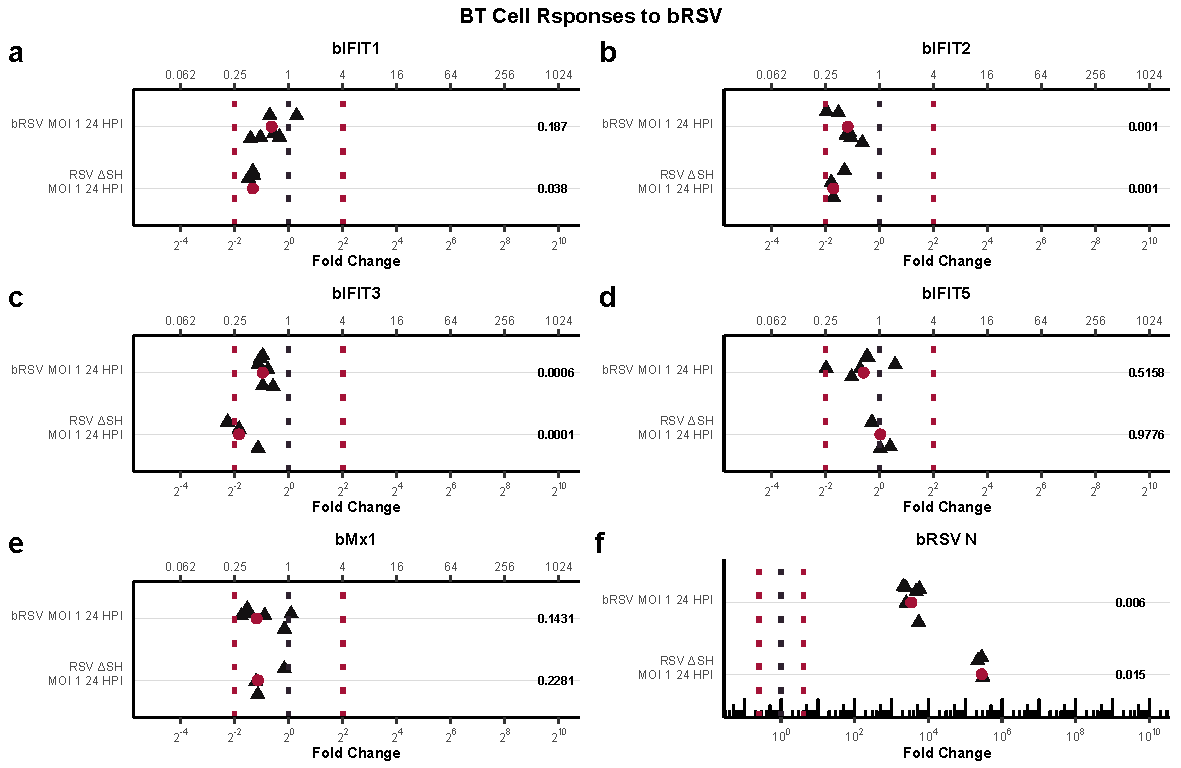
\includegraphics[width=1\linewidth]{07. Chapter 2/Figs/02. Induction/09. bt_brsv.pdf}
    \caption[BT \textit{bIFIT} Response to WT and \(\Delta\)SH bRSV Infection.]{\textbf{BT \textit{bIFIT} Response to WT and \(\Delta\)SH bRSV Infection.} (a) \textit{bIFIT1}, (b) \textit{bIFIT2}, (c) \textit{bIFIT3}, (d) \textit{bIFIT5}, (e) \textit{bMx1}, and (f) \textit{bRSV N} gene expression levels were assessed using quantitative real-time PCR (qPCR) in BT cell line following infection with WT or \(\Delta\)SH bRSV at MOI 1 for 24 hours post-infection. Relative expression values are normalized to standardized mock-treated samples. Median values are represented by red circles. The black dotted line represents mock expression levels, while the red dotted lines indicate biologically significant induction thresholds. Numeric values indicate the p-values compared to mock-treated samples.}
    \label{fig:BT responses to bRSV}
\end{figure}

some text some text some text some text some text


\begin{figure}
    \centering
    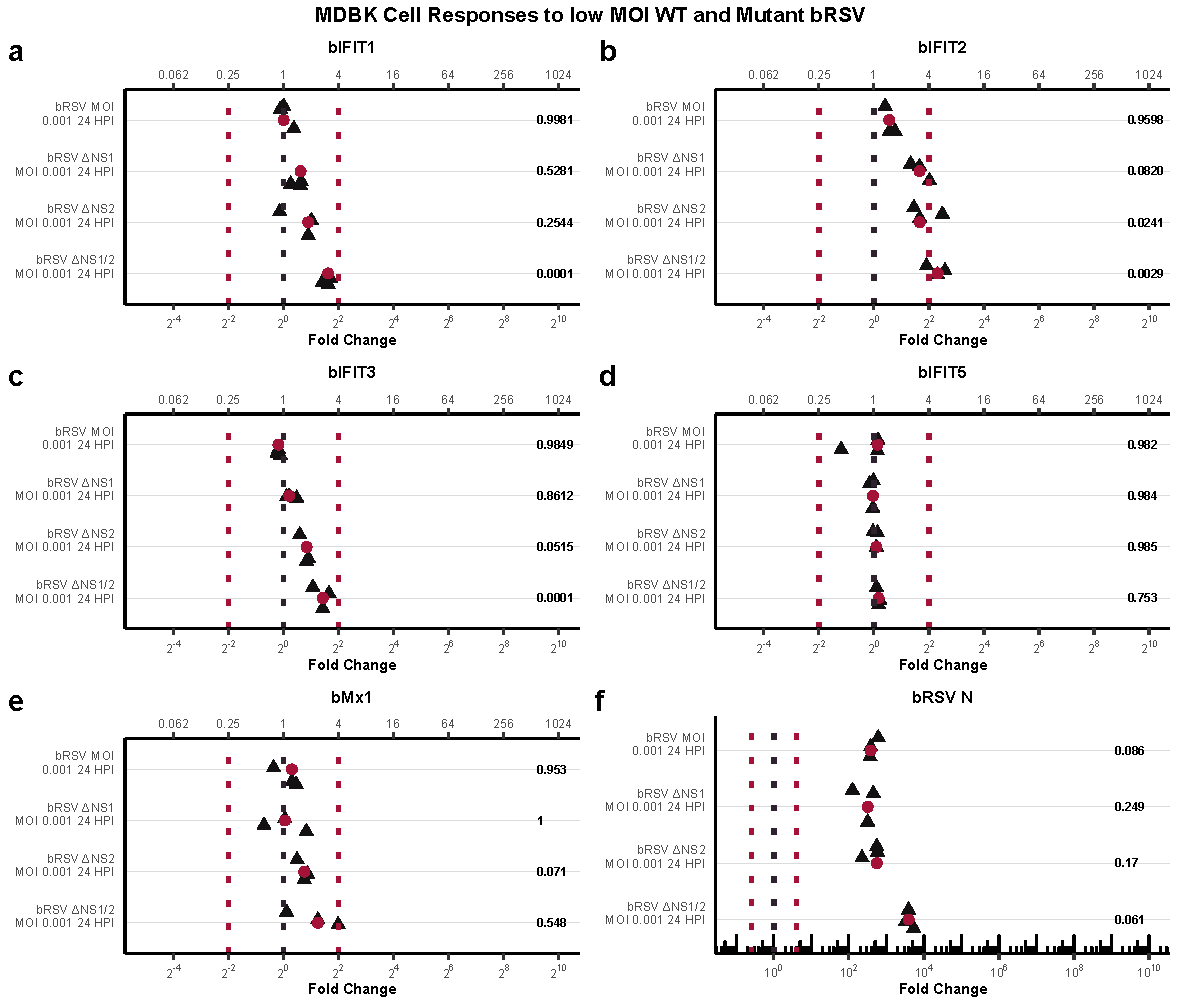
\includegraphics[width=1\linewidth]{07. Chapter 2/Figs/02. Induction/06. mdbk_brsv_low_moi.pdf}
    \caption[MDBK \textit{bIFIT} Response to Low MOI bRSV Infections.]{\textbf{MDBK \textit{bIFIT} Response to Low MOI bRSV Infections.} (a) \textit{bIFIT1}, (b) \textit{bIFIT2}, (c) \textit{bIFIT3}, (d) \textit{bIFIT5}, (e) \textit{bMx1}, and (f) \textit{bRSV N} gene expression levels were assessed using quantitative real-time PCR (qPCR) in MDBK cell line following infection with WT or \(\Delta\)NS1, \(\Delta\)NS2, and \(\Delta\)NS1/2 bRSV at MOIs of 0.001 for 24 hours post-infection. Relative expression values are normalized to standardized mock-treated samples. Median values are represented by red circles. The black dotted line represents mock expression levels, while the red dotted lines indicate biologically significant induction thresholds. Numeric values indicate the p-values compared to mock-treated samples.}
    \label{fig:MDBK responses to low MOI mutant bRSV}
\end{figure}

some text some text some text some text some text

\subsection{Bovine \textit{IFITs} Responses to hRSV} \label{subsec:Bovine IFITs Responses to hRSV}

Data show that ultracentrifugation purified hRSV causes no response in terms of bIFIT induction. Infection with normally purified virus does not cause induction either but hints at downregulation actually.

\begin{figure}
    \centering
    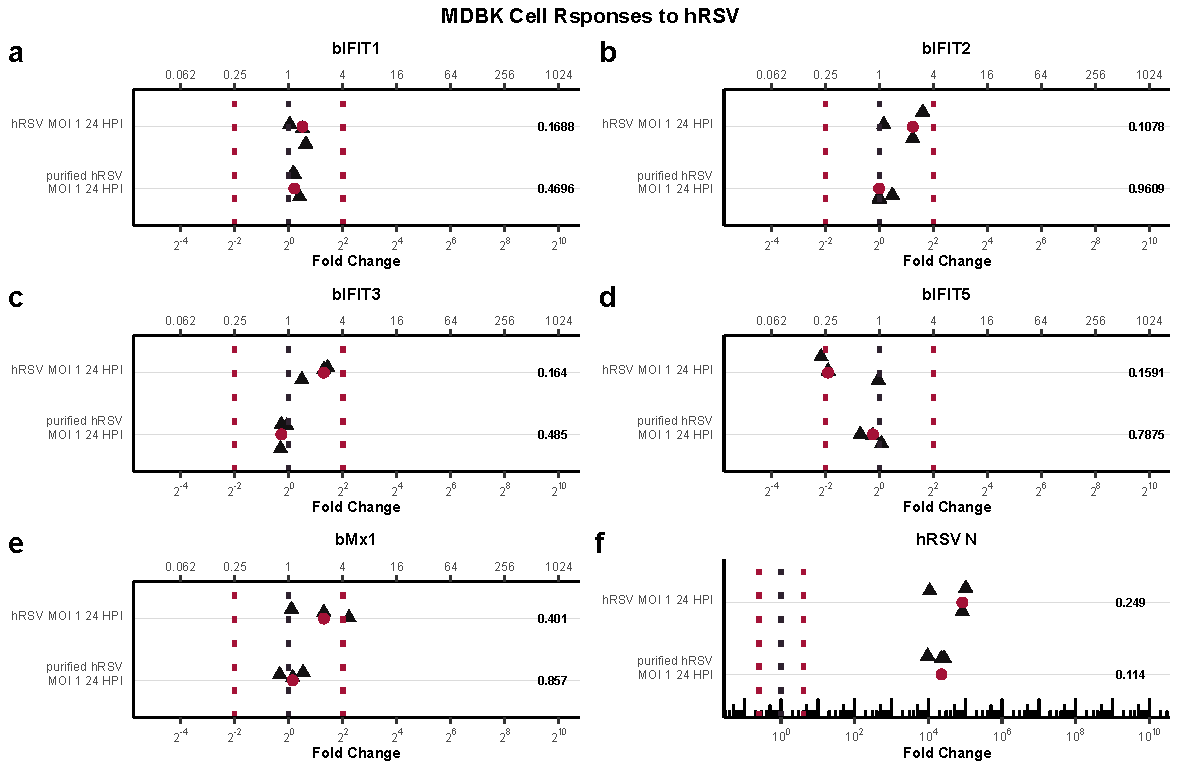
\includegraphics[width=1\linewidth]{07. Chapter 2/Figs/02. Induction/07. mdbk_hrsv.pdf}
    \caption[MDBK \textit{bIFIT} Response to Crude-Extracted and Ultra-Purified hRSV Infection.]{\textbf{MDBK \textit{bIFIT} Response to Crude-Extracted and Ultra-Purified hRSV Infection.} (a) \textit{bIFIT1}, (b) \textit{bIFIT2}, (c) \textit{bIFIT3}, (d) \textit{bIFIT5}, (e) \textit{bMx1}, and (f) \textit{hRSV N} gene expression levels were assessed using quantitative real-time PCR (qPCR) in MDBK cell line following infection with crude-extraccted and ultra-purified hRSV at MOI 1 for 24 hours post-infection. Relative expression values are normalized to standardized mock-treated samples. Median values are represented by red circles. The black dotted line represents mock expression levels, while the red dotted lines indicate biologically significant induction thresholds. Numeric values indicate the p-values compared to mock-treated samples.}
    \label{fig:bIFIT responses to hRSV infection in MDBK}
\end{figure}

some text some text some text some text some text

\begin{figure}
    \centering
    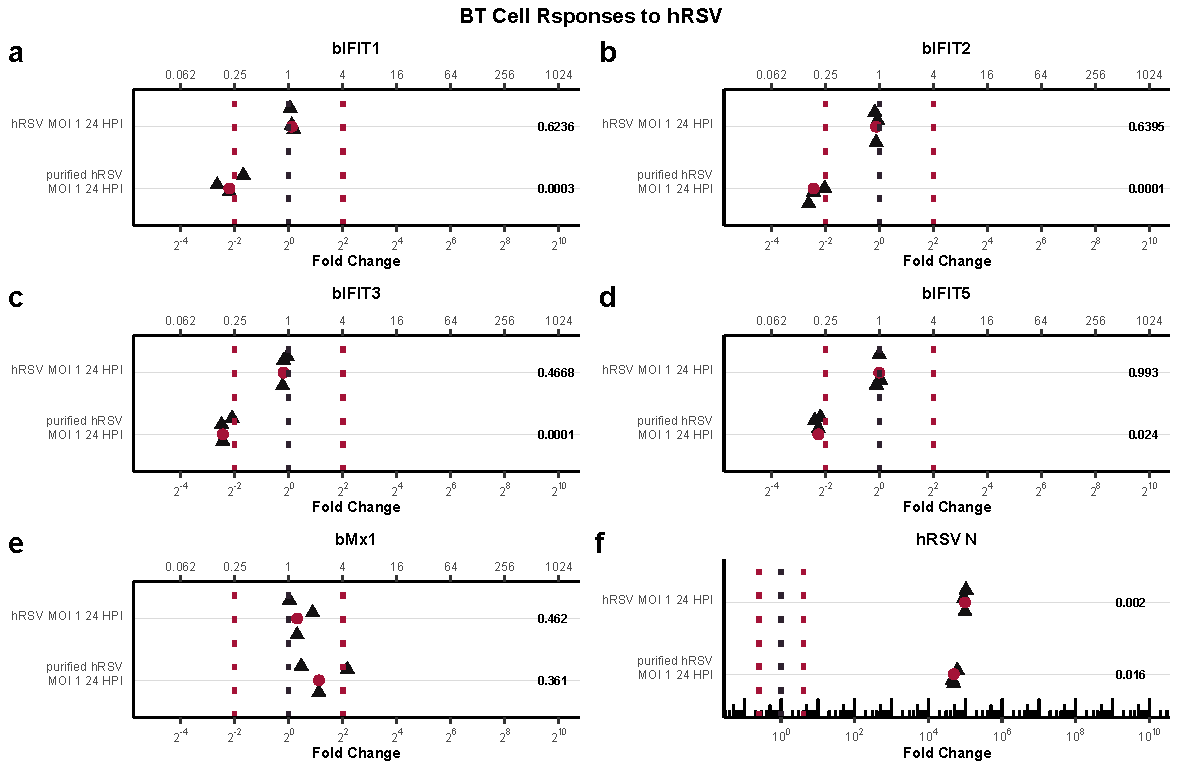
\includegraphics[width=1\linewidth]{07. Chapter 2/Figs/02. Induction/10. bt_hrsv.pdf}
    \caption[BT \textit{bIFIT} Response to Crude-Extracted and Ultra-Purified hRSV Infection.]{\textbf{BT \textit{bIFIT} Response to Crude-Extracted and Ultra-Purified hRSV Infection.} (a) \textit{bIFIT1}, (b) \textit{bIFIT2}, (c) \textit{bIFIT3}, (d) \textit{bIFIT5}, (e) \textit{bMx1}, and (f) \textit{hRSV N} gene expression levels were assessed using quantitative real-time PCR (qPCR) in BT cell line following infection with crude-extraccted and ultra-purified hRSV at MOI 1 for 24 hours post-infection. Relative expression values are normalized to standardized mock-treated samples. Median values are represented by red circles. The black dotted line represents mock expression levels, while the red dotted lines indicate biologically significant induction thresholds. Numeric values indicate the p-values compared to mock-treated samples.}
    \label{fig:Bt responses to hRSV}
\end{figure}


Describe data: \newline
asdasdas

Validation in more physiologically relevant cell line. All genes but bIFIT2 respond to bIFN alpha 5 ng/mL for 3h; treatment for 24h cause no change in any of the genes; treatment for 6h downregulates IFITs but not bMx1. This shows that BT cells are responsive to IFN and have the capability to express bIFITs and bMx1.

Ultracentrifugation purified hRSV causes downregulation in IFITs but not bMx1 (where it causes no change), while infection with normally extracted hRSV cause no change in none of the genes tested. Infections with wt bRSV and dSH bRSV at the same MOI and HPI (1 and 24) cause slight downregulation in all genes tested.

The trends seen with MDBK are kind of recapitulated.

